\section{Tool design}
\label{sec:contribution}

As explained previously, our tool design comprises three models: An integrated \textbf{data model}, a \textbf{permission model}, and an \textbf{interface model}.
The integrated data model describes our representation of stakeholders, roles, CAD model revisions, design tasks, and project schedules.
The permission model explains which changes the individual stakeholders can perform on top of the data model depending on his/her role.
Finally, the interface model demonstrates how the previous models can be put into action practically.

\subsection{Data model}

\begin{figure*}[ht]
    \centering
    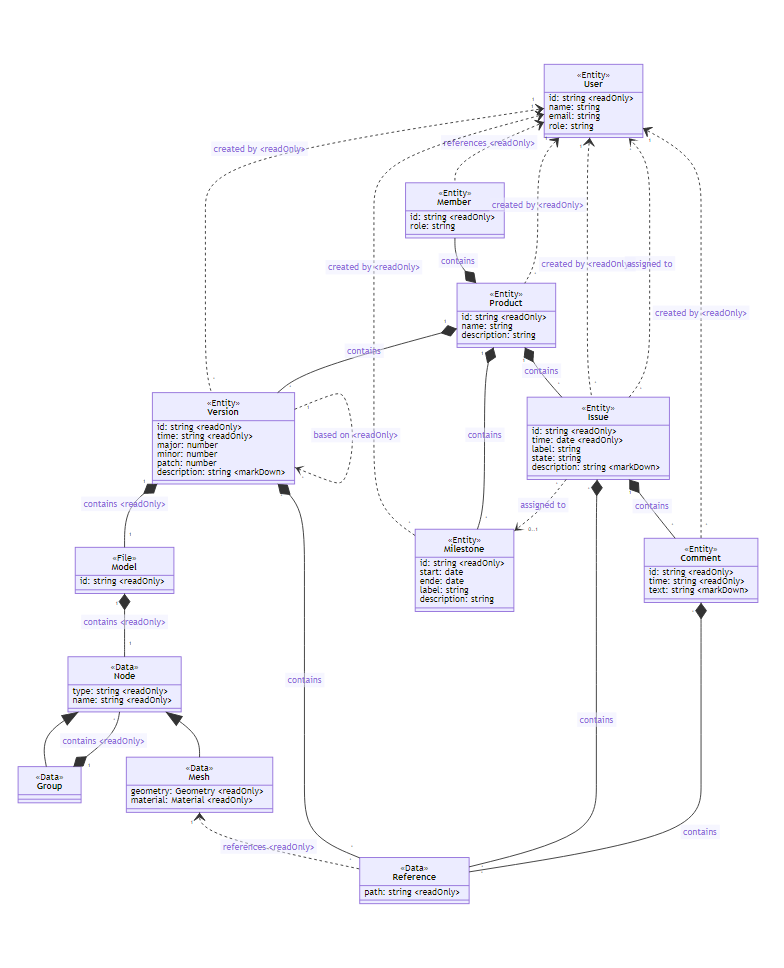
\includegraphics[width=\textwidth]{entities-v5.png}
    \caption{Integrated data model for improved information exchange between customers, project managers, requirements engineers, and product designers}
    \label{fig: datamodel}
\end{figure*}

This section describes the integrated data model as shown in Figure~\ref{fig: datamodel}.
The data model contains the following entities: \textit{User}, \textit{Product}, \textit{Version}, \textit{Issue}, \textit{Comment}, \textit{Milestone}, and \textit{Member}.
Note that all entities share a common identifier attribute, which is used for referencing and linking entities.
Furthermore, all entities share a common deleted attribute, which is used to hide entities from the users after removal.

% User
The \textit{User} entity represents the individual stakeholders, who access the tool during product development.
The entity defines an email and a password attribute, which are used for authentication purposes.
Additionally, the entity defines a name attribute, which is used for a human-readable identification of stakeholders.
Similarly, the entity links an \textit{Image} file, which provides a human-interpretable visual representation of stakeholders (i.e.\ a profile picture).
Furthermore, the entity defines a user manager and a product manager flag, which are used for permission control as explained later.

% Product
The \textit{Product} entity represents the individual products or product development projects managed with the tool.
The entity is always linked to a \textit{User} entity, representing the stakeholder who created the product in the first place.
Then, the entity defines a name attribute, which is used to identify the product in a human-readable manner.
Furthermore, the entity defines a description attribute, which is used to explain the purpose of the product only briefly.

% Member
The \textit{Member} entity represents the permission to access certain product data through the tool.
Consequently, the entity is linked to a \textit{Product} entity, representing the product for which access is granted.
Also, the entity is linked to a \textit{User} entity, representing the stakeholder who is granted product access.
Finally, the entity defines a \textit{role} attribute, which controls the permission level as explained later, and which can have one of three values: \textit{manager}, \textit{engineer}, or \textit{customer}.

% Version
The \textit{Version} entity represents a revision of the product design created by a product designer.
The entity is linked to a \textit{Product} entity to identify the product, for which the design revision was created.
Similarly, the entity is linked to a \textit{User} entity to identify the product designer, who was responsible for creating the design revision.
Furthermore, the entity is linked to previous \textit{Version} entities to document the history of design revisions including version branching and merging.
Then, the entity defines a major, a minor, and a patch number, which together represent a version number according to semantic versioning\footnote{\url{https://semver.org/}} practices.
Also, the entity defined a description, which provides a human-readable explanation of the design changes that have been applied.
Finally, the entity links a \textit{Model} file, which represents the actual design data including assembly and part structures as well as geometry and material information.

% Model
We work with a generic representation of \textit{Model} files, which is independent of the CAD tool vendor and data format used.
We assume a model contains \textit{Node} objects, which carry all the engineering information created by the product designer.
Furthermore, we assume a node defines a name attribute, which can be used as for human-readable identification of nodes.
Additionally, we assume a node provides a type attribute, which can be used to distinguish different types of nodes.
At the moment, we distinguish two types of nodes, namely \textit{Group} nodes and \textit{Mesh} nodes.
Groups represent the assembly structures and provide links to child nodes being assembled, which can be both groups and meshes.
Meshes, on the other hand, represent the atomic parts of the product design such as screws or rivets, and carry geometry and material information.
Technically, we work with the glTF\footnote{\url{https://www.khronos.org/gltf/}} format for representing models including their node structures as well as their geometry and material information.
However, the STEP\footnote{\url{https://www.iso.org/standard/66654.html}} format or the COLLADA\footnote{\url{https://www.khronos.org/collada/}} format could be used equally well, since they follow the same principles.
In fact, even a vendor-specific data format could be used as long as appropriate parsers are available.

% Milestone
The \textit{Milestone} entity essentially represents project schedules including deadlines for the realization of design tasks.
The entity always links a \textit{Product} entity to identify the product or project the milestone belongs to.
Furthermore, the entity links a \textit{User} entity to identify the product manager, who created the milestone.
Finally, the entity defines a start and an end date, which represent the time frame for working on the milestone and achieving its goals.

% Issue
The \textit{Issue} entity represents design tasks, which have to be performed by product designers during product development projects.
The entity is always linked to a \textit{Product} entity to identify the product or project the issue belongs to.
Furthermore, the entity is linked to multiple \textit{User} entities to identify the one stakeholder, who reported the issue in the first place, and to identify the product designers, who are responsible for issue resolution.
Moreover, the entity can be linked to a \textit{Milestone} entity to identify the time frame, within which the issue should be resolved.
Then, the entity defines a time attribute, which records the point in time when the issue was reported originally.
Also, the entity defines a label attribute, which provides a human-readable summary of the issue.
Additionally, the entity defines a text attribute, which provides a more detailed explanation of the design task including markdown-based\footnote{\url{https://www.markdownguide.org/}} \textit{Reference} objects as explained later.
Finally, the entity defines a state attribute, which enables us to distinguish between open and closed design tasks.

% Comment
The \textit{Comment} entity represents discussions between stakeholders on issues or design tasks respectively.
The entity links an \textit{Issue} entity to identify the issue or design task the comment belongs to.
Furthermore, the entity links a \textit{User} entity to identify the stakeholder, who posted the comment.
Then, the entity defines a time attribute, which records the point in time when the comment was posted.
Additionally, the entity defines a text attribute, which contains the actual content of the comment including markdown-based \textit{Reference} objects as explained later.
Finally, the entity defines an action attribute, which can be used to close or reopen an issue by posting a comment.

% Reference
As explained previously, we work with a markdown-based representation of \textit{Reference} objects, which can be contained in the description of \textit{Issue} entities as well as \textit{Comment} entities.
These references can be used to refer to \textit{Node} objects, that are contained in the CAD models of design revisions for a particular product or project.
Consequently, the specification and discussion of design tasks can be enriched with links to assembly structures and parts, which have been designed and delivered previously.
%\subsection{Permission model}

\label{subsec:permissionModel}
The permission model offers a number of possible restrictions on the platform so that not every user has all freedoms. This is especially important when cooperating with customers. The customer should only have the possibility to evaluate existing products. For this he can see the products he is registered for and use the given product management functions depending on its member role \textit{customer}. Creating new users and products should only be possible by the managers of the respective product. They also organize the rights of each user. The permission model is divided into two levels. The first level is the global level and the second level is the product level. The global level uses a permission model and the product level a role model which is implicitly linked to the permission model. 
This allows the first level to manage products and users and the role model to distribute more specific permissions to the individual products. This system is deeply integrated in the backend.

\subsubsection{Global level}

The \textit{User} entity has the two attributes \textit{user management permission} and \textit{product management permission}. Only a user who has the user management permission can create or edit users. On the other hand every user can edit his own personal data. With the product management permission it is possible to create new products. If a new product is created, the respective user is automatically also a product member and receives the member role \textit{manager}. The permissions of each user can be adjusted afterwards. So it is possible to give multiple users the permissions for user management and product management. For example, a user and product manager can exist for each department. 

\subsubsection{Product level}

For permission management at product level, three member roles are provided. These roles are: \textit{manager, engineer and customer}. The manager is the one who created the product and has the permission to add more members. So he can add more managers, who in turn have all the rights over the management of the product. This is useful when the product development covers several departments. The second role is the engineer. He is involved in the product development process. He has no rights to change the product description or its members. However, he can freely create and edit versions, issues and comments. The last role is the customer who has the possibility to observe the product development process. He can create issues and comments and so participate in the product development process. In the current version of the software the rights of the customer are still very strict. The permission system is implemented in such a way that it can be changed with few adjustments. If the customer needs writing permissions, this can be easily changed.
\subsection{Interface model}

The user interface provides a convenient way to interact with the functional model to display and modify data. The user interface offers a consistent design, which runs through the entire system.

\subsubsection*{Product view}

The \textit{product view} page lists all available products, for which the user has the permission to see them, in a table [see Fig. \ref{fig: startpage} on page~\pageref{fig: startpage}]. For each product in the table a preview is shown. The other columns show the attributes \textit{owner, name, description, versions, issues and members}. The X on the right provides the possibility to delete the corresponding product. The owner is the person who created the product. Name and description are defined when the product is created and can be changed later. The columns on the right show how many versions exist for this product, how many issues have been created and how many members have access to the product. By clicking on New product you get also to the ProductSettings view where you can add a new product when you have the product management permission. This button is only visible when the corresponding user has product management permission. The CAD model and version details will be added when the user creates a new version of a product.

\begin{figure}[h]
    \centering
    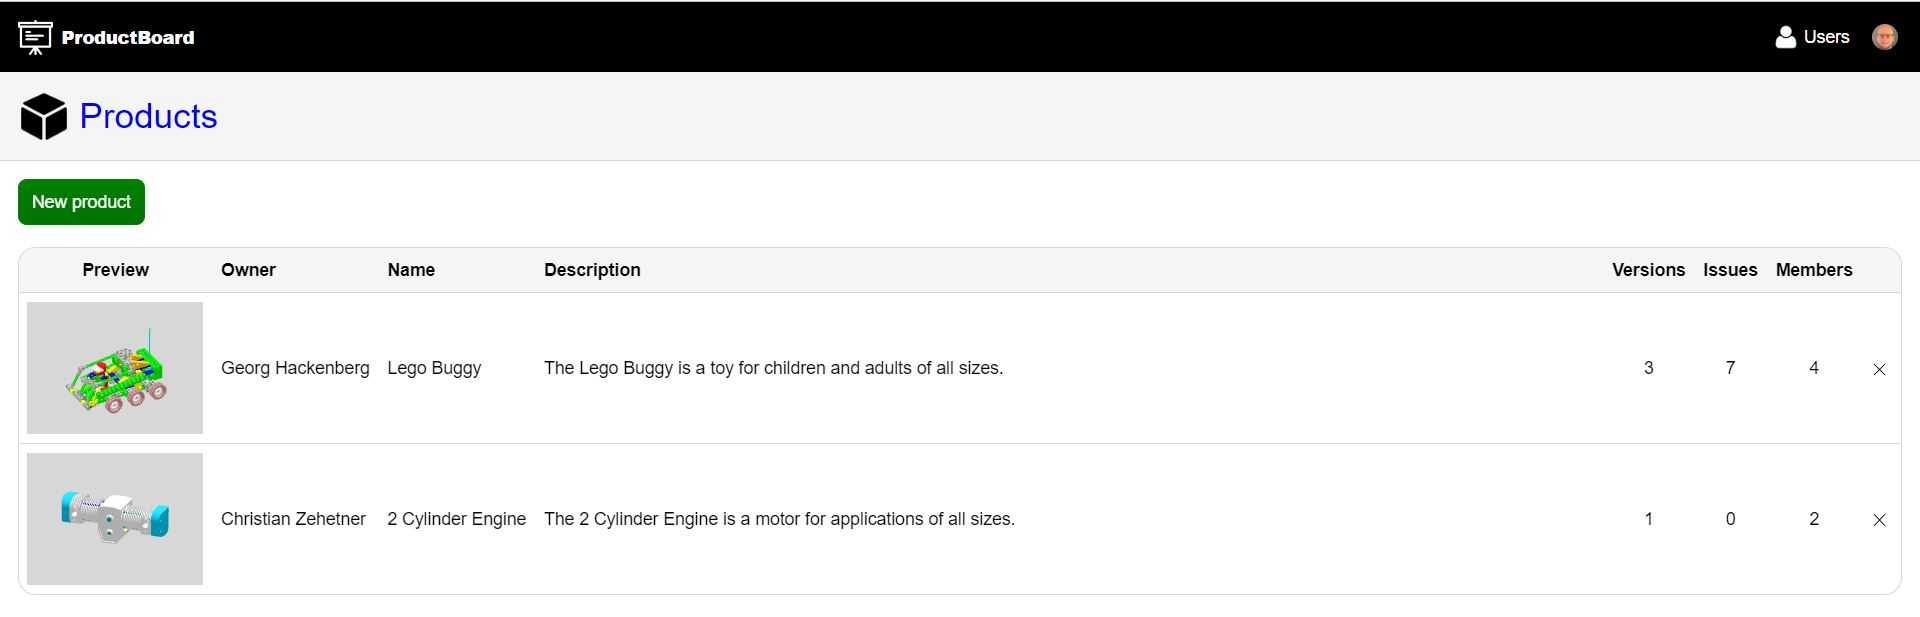
\includegraphics[width=\columnwidth]{startpage.JPG}
    \caption{Product view}
    \label{fig: startpage}
\end{figure}

\subsubsection*{ProductVersion view}

Clicking on a product takes you to the ProductVersion view. You can also use the toolbar to jump to other pages such as issues, milestones members or settings. The left side of the view shows the created versions. On the left side there is a tree structure similar to GitHub. This tree structure results from the chronological arrangement of the product versions. The lines of the structure show how the product versions are in relation to the respective base versions. In the middle is the corresponding version number with the owner of the version inclusive email and a short description. Each version offers a preview. By clicking on the respective version, the 3D view on the right side also changes and shows the selected model. The 3D view allows to rotate, move and zoom the model. 
With a click on the \textit{New version} button you get to the ProductVersionSettings view where you can create new product versions. [see Fig. \ref{fig: versionsettingsview} on page~\pageref{fig: versionsettingsview}]. 

\subsubsection*{ProductVersionSettings view}

Here you can enter information for a new version and select an GLB file. Depending on the selected base versions, the ProductVersion view shows the new version with the corresponding new tree structure after pressing the Save button. It is also possible to select multible base versions to merge them into a new version.

\begin{figure}[h]
    \centering
    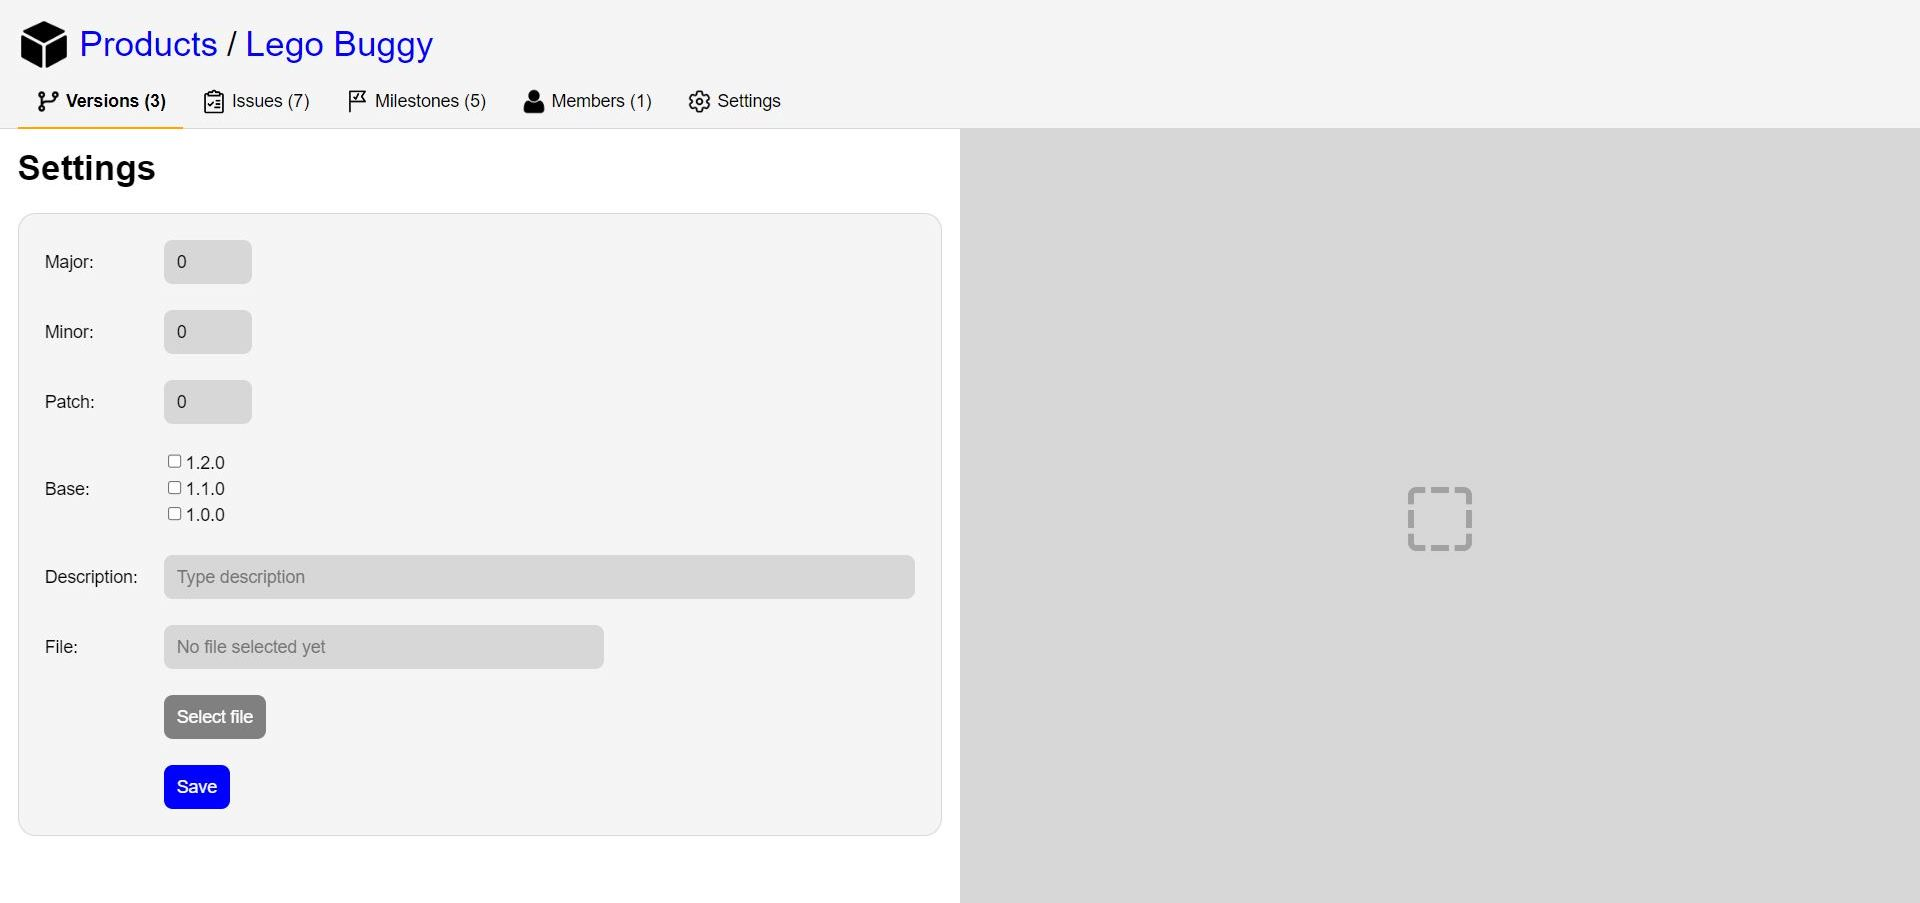
\includegraphics[width=\columnwidth]{versionsettingsview.JPG}
    \caption{ProductVersionSettings view}
    \label{fig: versionsettingsview}
\end{figure}

\subsubsection*{ProductIssue view}

By clicking on the Issues link, you access the ProductIssue view [see Fig. \ref{fig: issueview} on page~\pageref{fig: issueview}]. Here the created issues are displayed in a table. The two buttons Open Issues and Closed Issues can be used to filter the list accordingly. The table shows the reporter who created the issue, the associated label, the assignees and how many comments and marked parts are in the conversation channel. 
All views with 3D View offer the possibility to select a desired version for viewing. In the version view the version can be clicked directly. In the other views the version can be selected via a dropdown menu. This menu is located in the upper left corner of the 3D View. 
If the user hovers with the mouse over a part of the 3D model, this part gets highlighted. 
When hovering over an issue, the 3D view shows those parts that have been referenced in the comments of the respective issue by highlighting them in red.
When hovering over an issue the parts are only highlighted if the version on which the parts were selected was picked in the dropdown menu. Thats because the 3d view shows for each version only the markers that were created on corresponding version.

\begin{figure}[h]
    \centering
    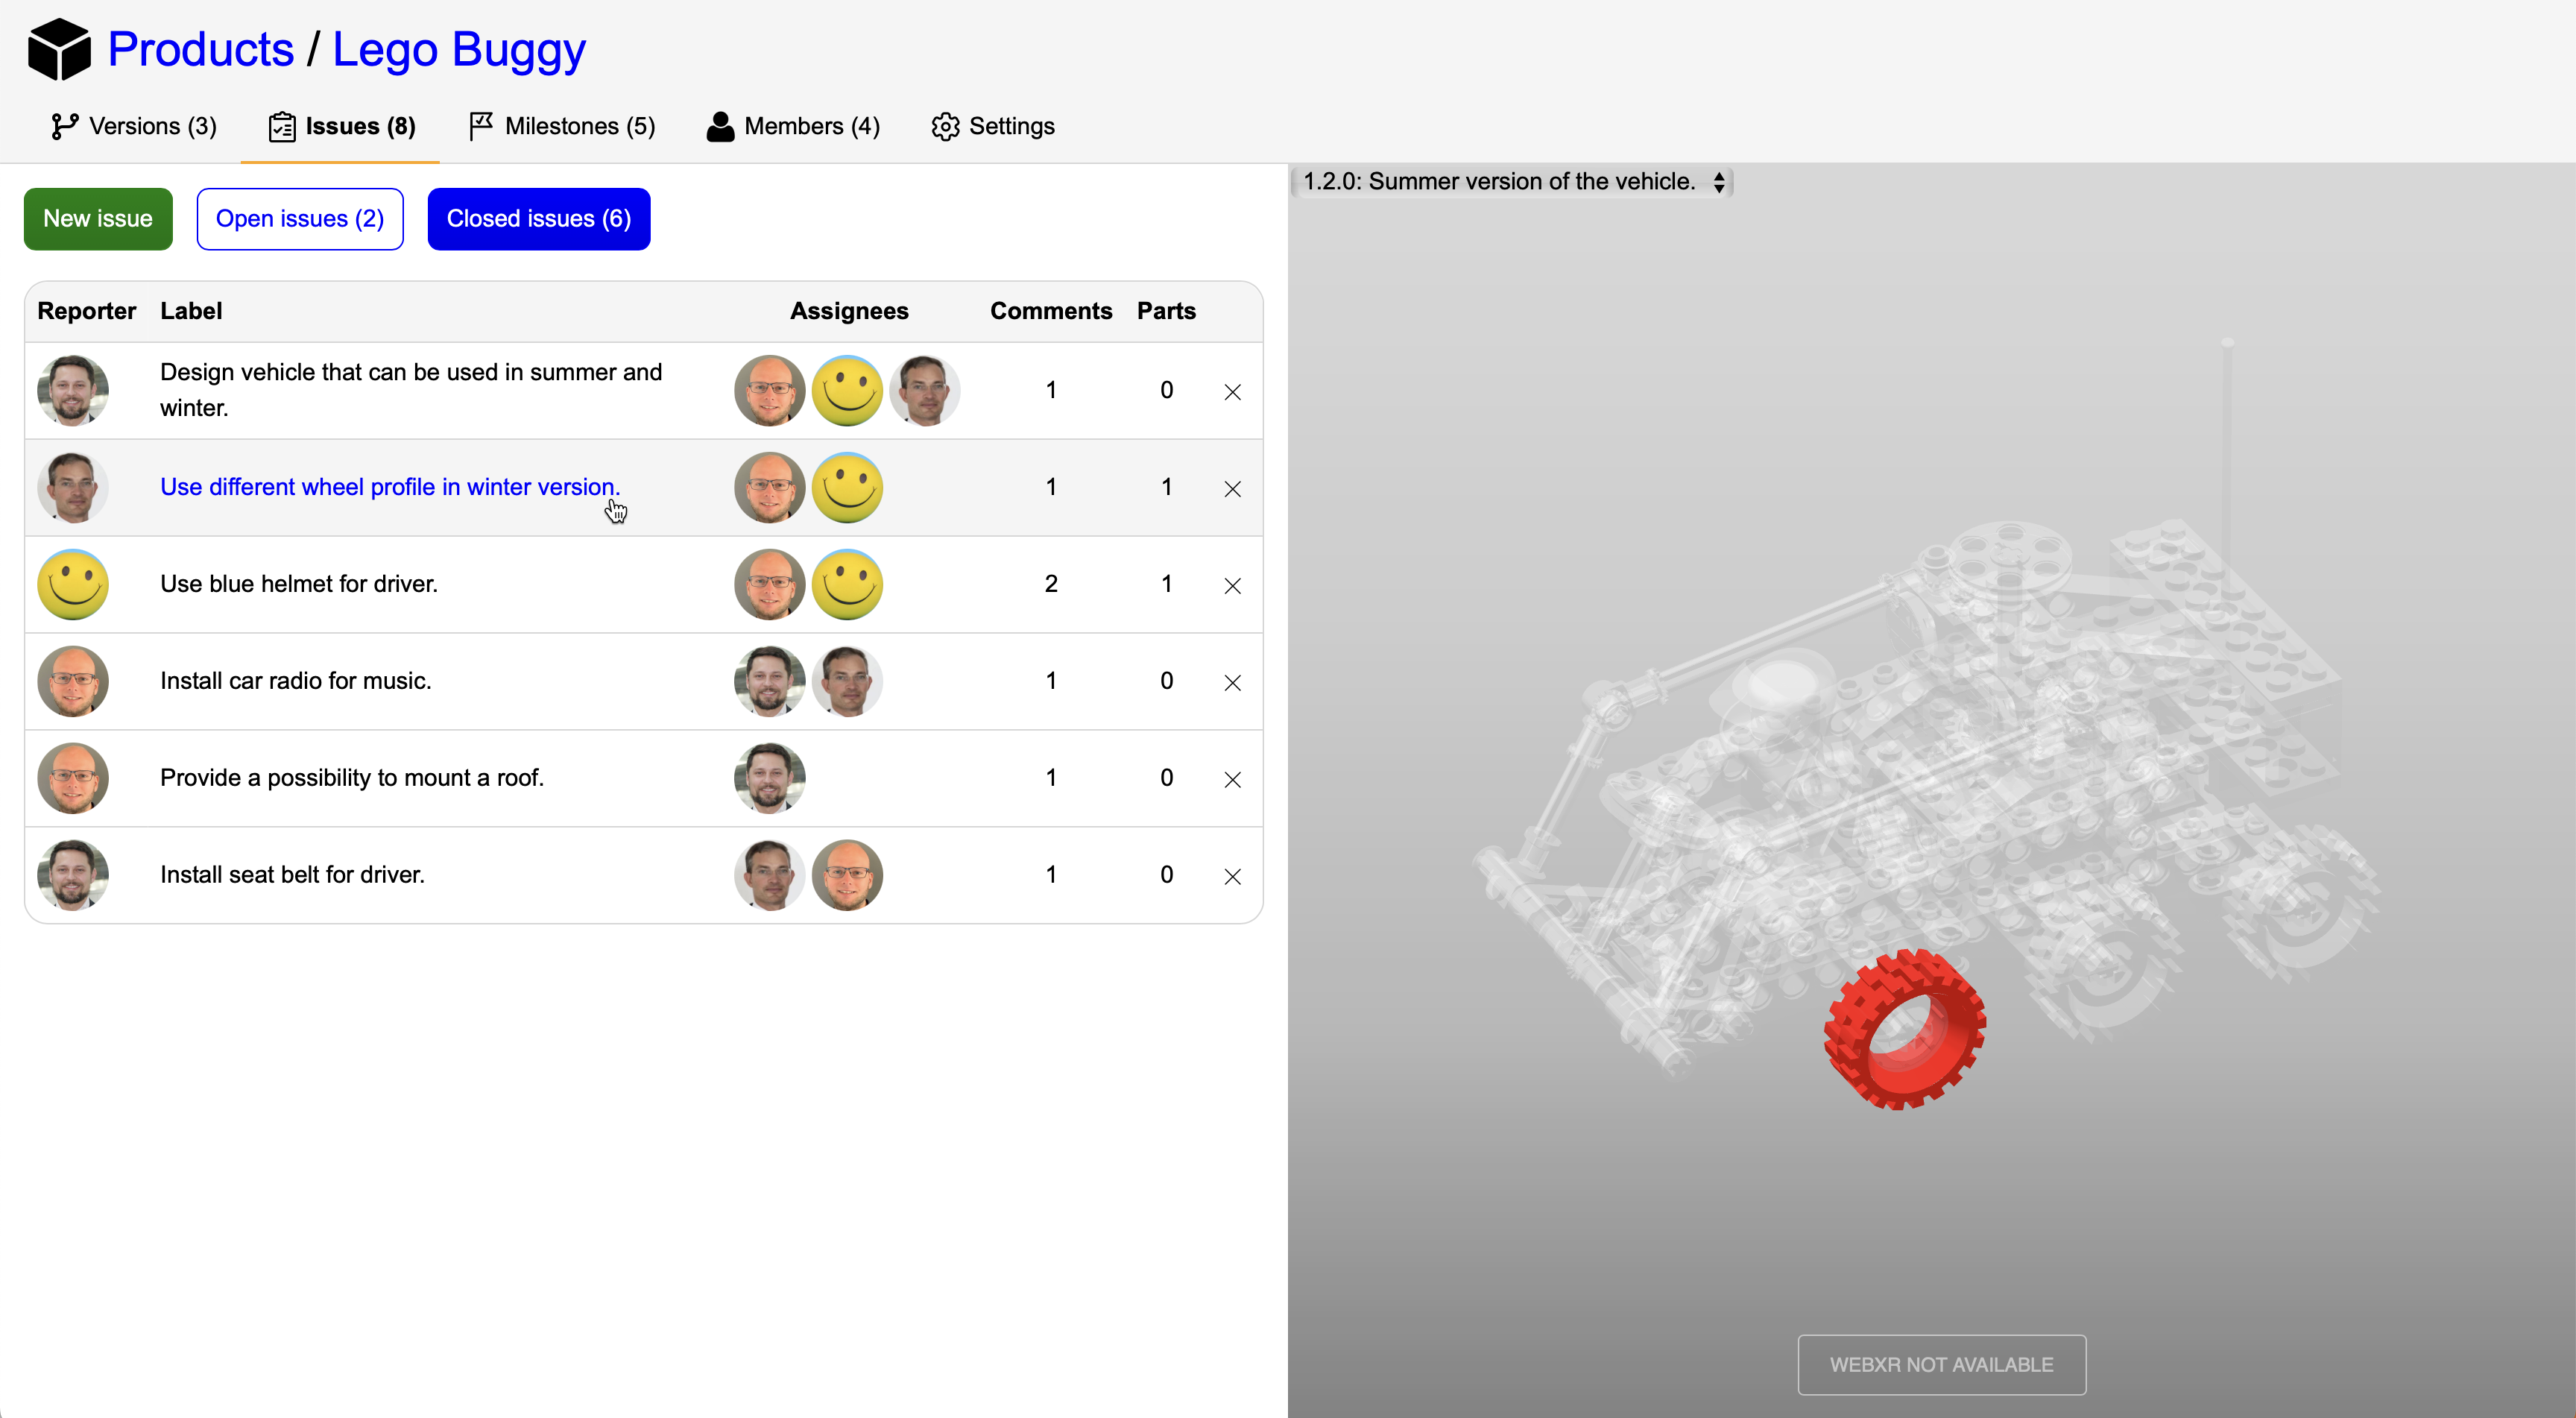
\includegraphics[width=\columnwidth]{issueviewselectedpart.png}
    \caption{Issue view}
    \label{fig: issueview}
\end{figure}

\subsubsection*{ProductIssueSettings view}

The ProductIssueSettings view allows to create new issues for the product [see Fig. \ref{fig: issuesettingsview} on page~\pageref{fig: issuesettingsview}]. The label, the text, the milestone and the assignees can be defined. An existing milestone can be selected with the dropdown menu. An issue must not be assigned to a milestone. This choice lies by the user. 
As in the ProductIssue view, the model of the desired version can also be selected here via dropdown menu on the 3D view.
The \textit{text} field in the ProductIssueSettings view represents the first comment in an issue. By clicking on the part, the part gets included in the comment as markdown text. If a comment includes a marked part when created, the marking of the respective part is saved to the associated product version.
The Save button closes the settings, and you return to the ProductIssue view where the new issue is visible.

\begin{figure}[h]
    \centering
    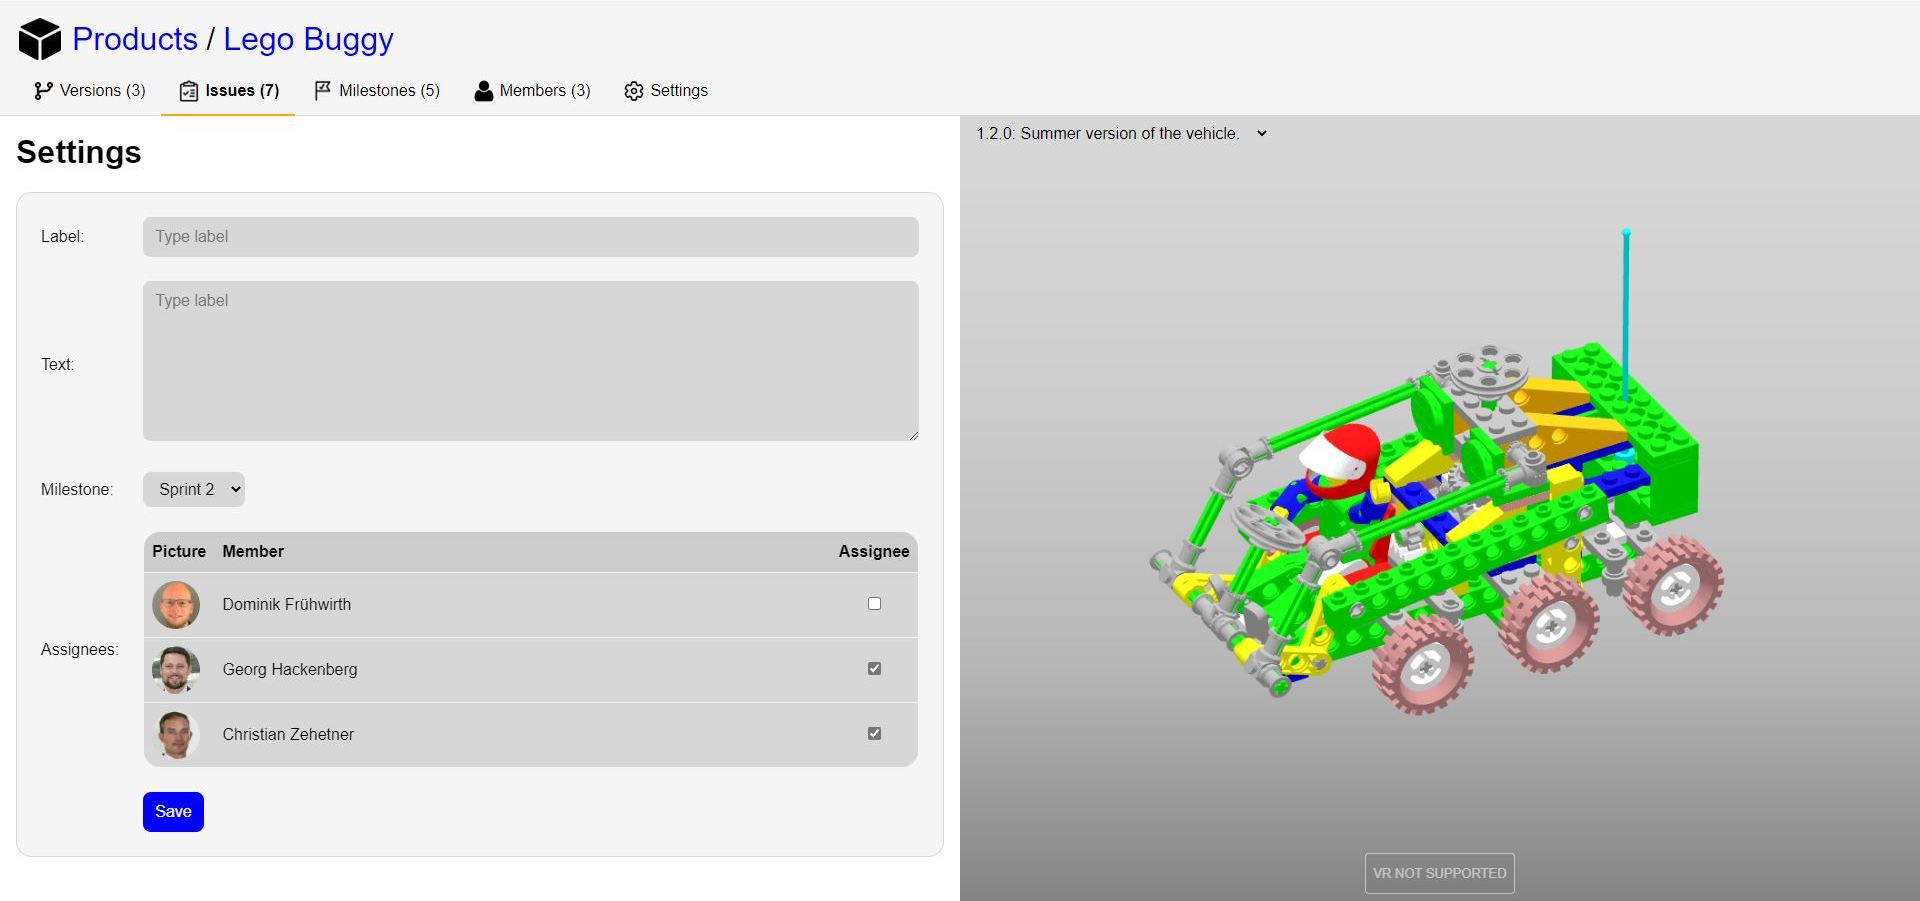
\includegraphics[width=\columnwidth]{issuesettingsview.JPG}
    \caption{Issuesettings view}
    \label{fig: issuesettingsview}
\end{figure}

\subsubsection*{ProductIssueComment view}

Clicking on an issue in the Issue view opens the corresponding ProductIssueComment view.  Here you have the possibility to discuss the issue. 
For this purpose, in the new comment box a text can be entered. This text field supports markdown.
Like in the ProductIssueSettings view you can click on a part of the 3D model to mark a part as markdown[see Fig. \ref{fig: commentselectedpartview} on page~\pageref{fig: commentselectedpartview}]. In the course of a discussion, several parts can be marked in this way.
A comment can also be used to close an issue by clicking the close button. This issue will then be found in Closed Issues in the ProductIssue view. With the comment function it is also possible to reopen the issue in the same way. The Close button displays the text Reopen when an issue is closed. In the upper right corner of the ProductIssueComment view there is a button to edit the selected issue. For example, the issue can be assigned to another Milestone or other attributes like the label, text or the list of assignees can be changed [see Fig. \ref{fig: issuesettingsview} on page~\pageref{fig: issuesettingsview}].

\begin{figure}[h]
    \centering
    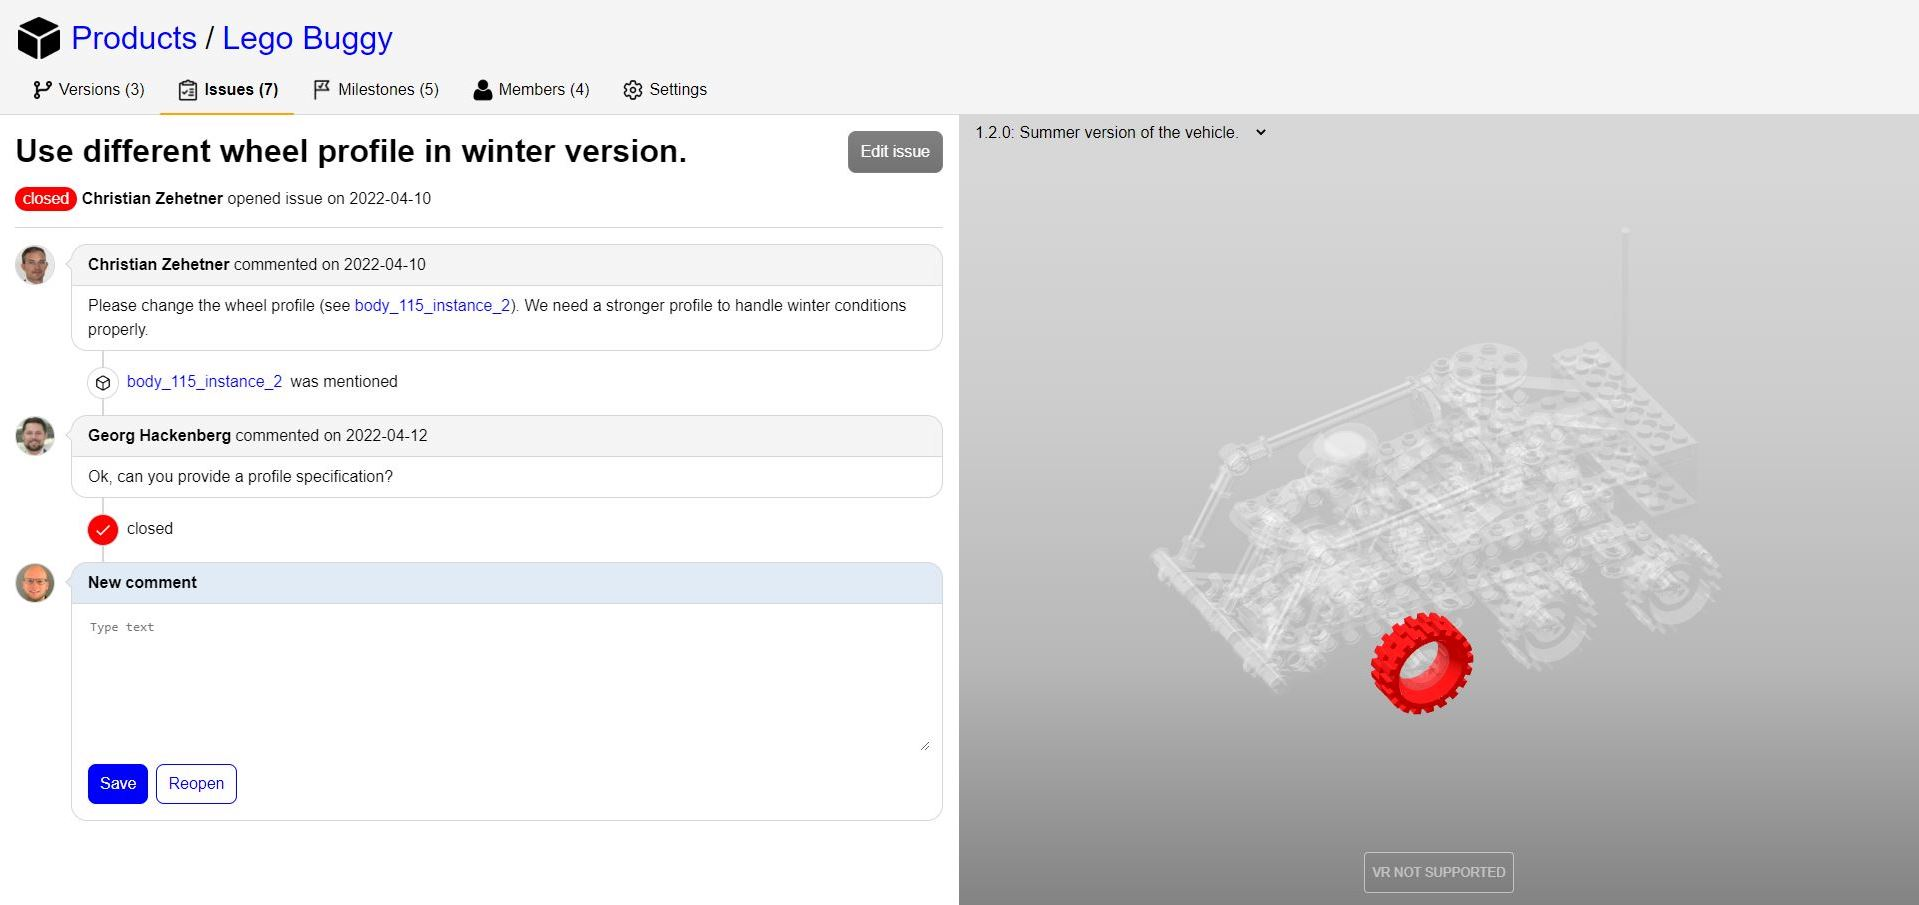
\includegraphics[width=\columnwidth]{commentselectedpartview.JPG}
    \caption{Selected part in ProductIssueComment view}
    \label{fig: commentselectedpartview}
\end{figure}

\subsubsection*{ProductMilestone view}

The ProductMilestone view can be accessed via the Milestones link [see Fig. \ref{fig: milestoneview} on page~\pageref{fig: milestoneview}]. A table shows who created the milestone, its name, start date, end date and the progress. For each milestone two progress bars are displayed. The first one shows the date progress of a milestone by calculating \textit{100 * (nowDate - startDate) / (endDate - startDate)}. The second bar shows the issue progress of a milestone by calculating \textit{100 * number of closedIssues / number of allIssues}.
A click on the New Milestone button leads to the ProductMilestoneSettings view. Here the attributes of a milestone can be adjusted and saved. The new or edited Milestone than show up in the ProductMilestone view.

\begin{figure}[h]
    \centering
    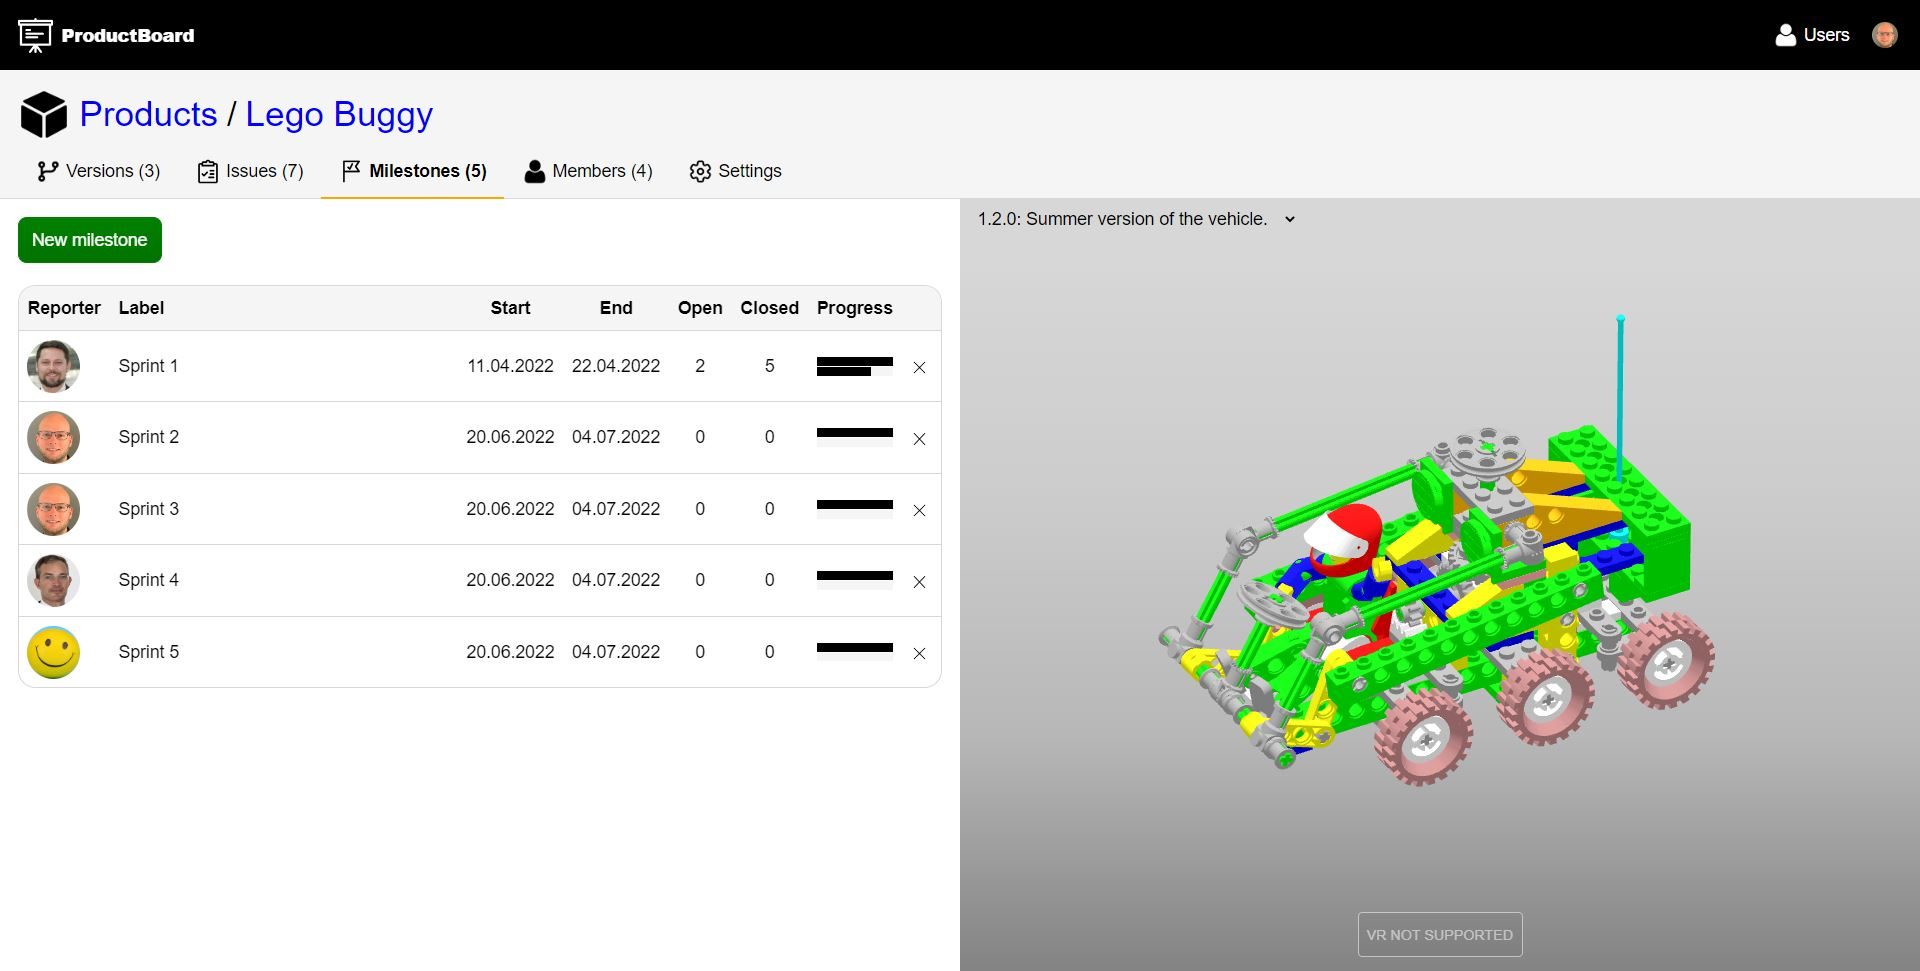
\includegraphics[width=\columnwidth]{milestoneview.JPG}
    \caption{ProductMilestone view}
    \label{fig: milestoneview}
\end{figure}

\subsubsection*{ProductMilestoneIssue view}

If a milestone is selected, a table with the attached issues is displayed [see Fig. \ref{fig: sprintview} on page~\pageref{fig: sprintview}]. This table is identical to the one in the ProductIssue view. Here you can also filter by open and closed issues. On the right side a burn down chart is displayed which shows the current progress of the milestone. The chart shows the start date, the end date, the number of issues and the progress until the current day. In the chart, the green line represents the target burndown and the blue graph the actual burndown. The target burndown distributes the open issues over the time span. The actual burndown drops by one for each issue that is closed.  Like in the ProductMilestone view, a click Edit Milestone button leads to the ProductMilestoneSettings view where the attributes of a milestone can be changed.

\begin{figure}[h]
    \centering
    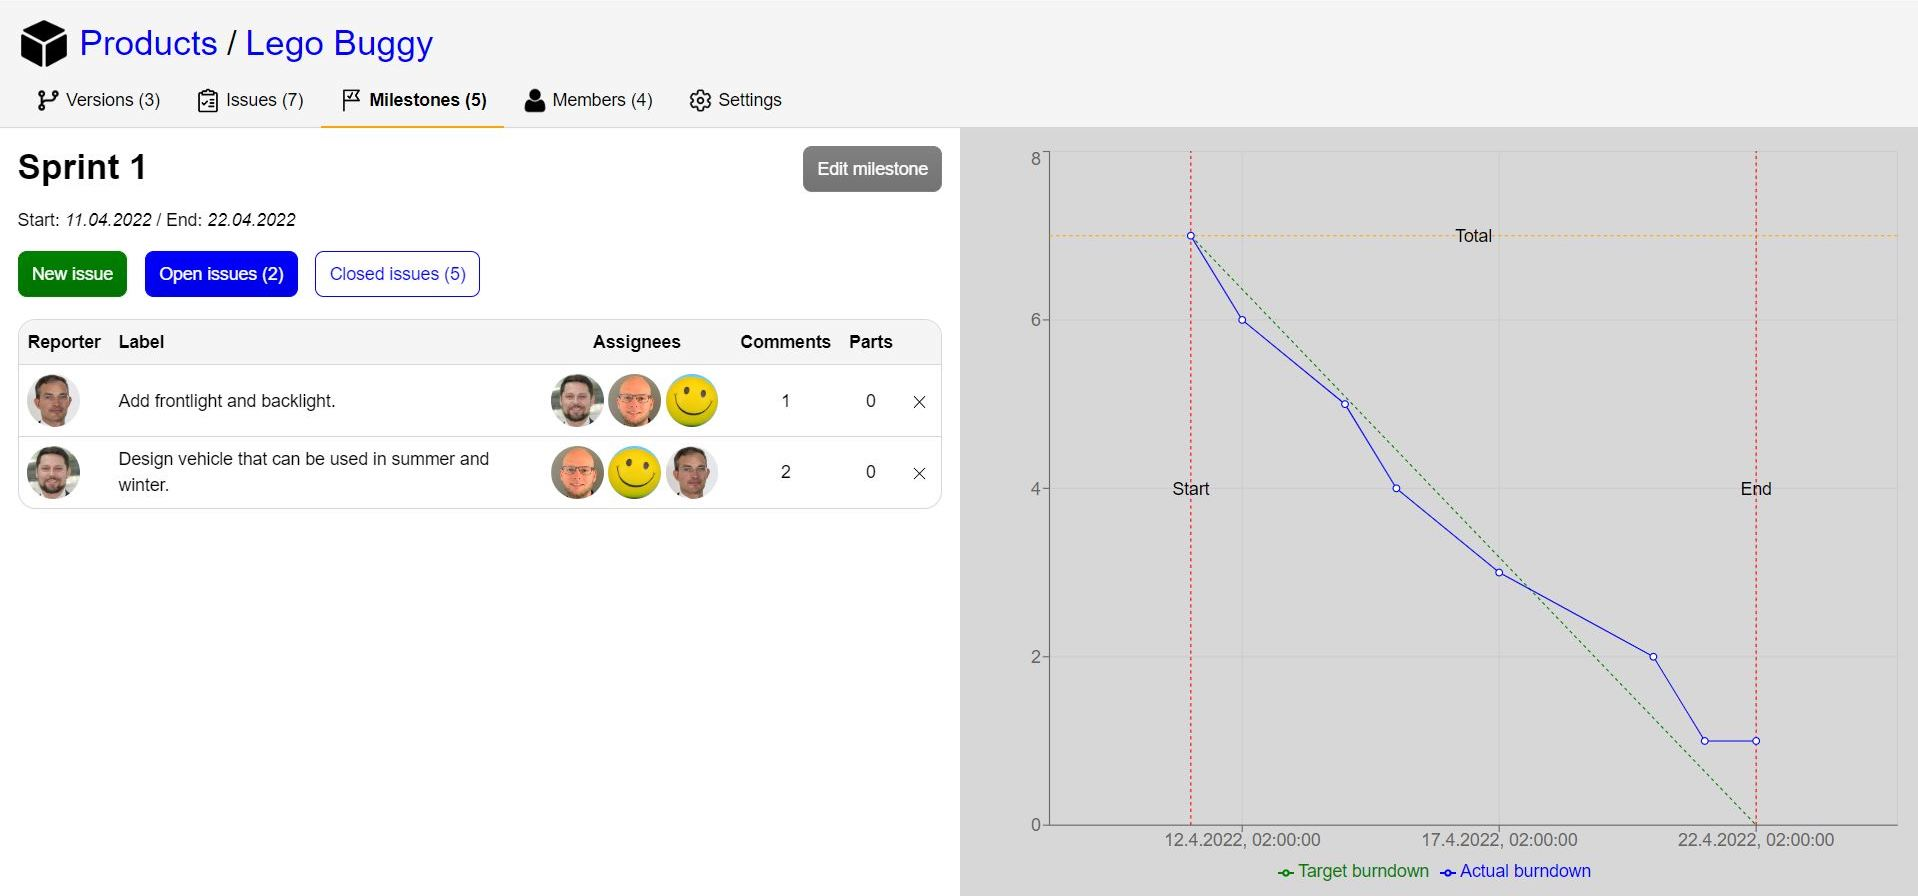
\includegraphics[width=\columnwidth]{sprintview.JPG}
    \caption{ProductMilestoneIssue view}
    \label{fig: sprintview}
\end{figure}

\subsubsection*{ProductMember view}

To distribute the rights for a product, members are added to an existing product via the user interface. In the ProductMember view, a table shows all members who have access to the selected product [see Fig. \ref{fig: memberview} on page~\pageref{fig: memberview}]. The table shows the user picture and the name of the user. The role column defines which rights the respective member has. At the moment there are three roles: \textit{manager, engineer, customer} as explained in the permission model.. As with every overview table, objects can be deleted from the list by clicking on the X button. The button New Member leads to the ProductMemberSettings view where new members can be added.

\begin{figure}[h]
    \centering
    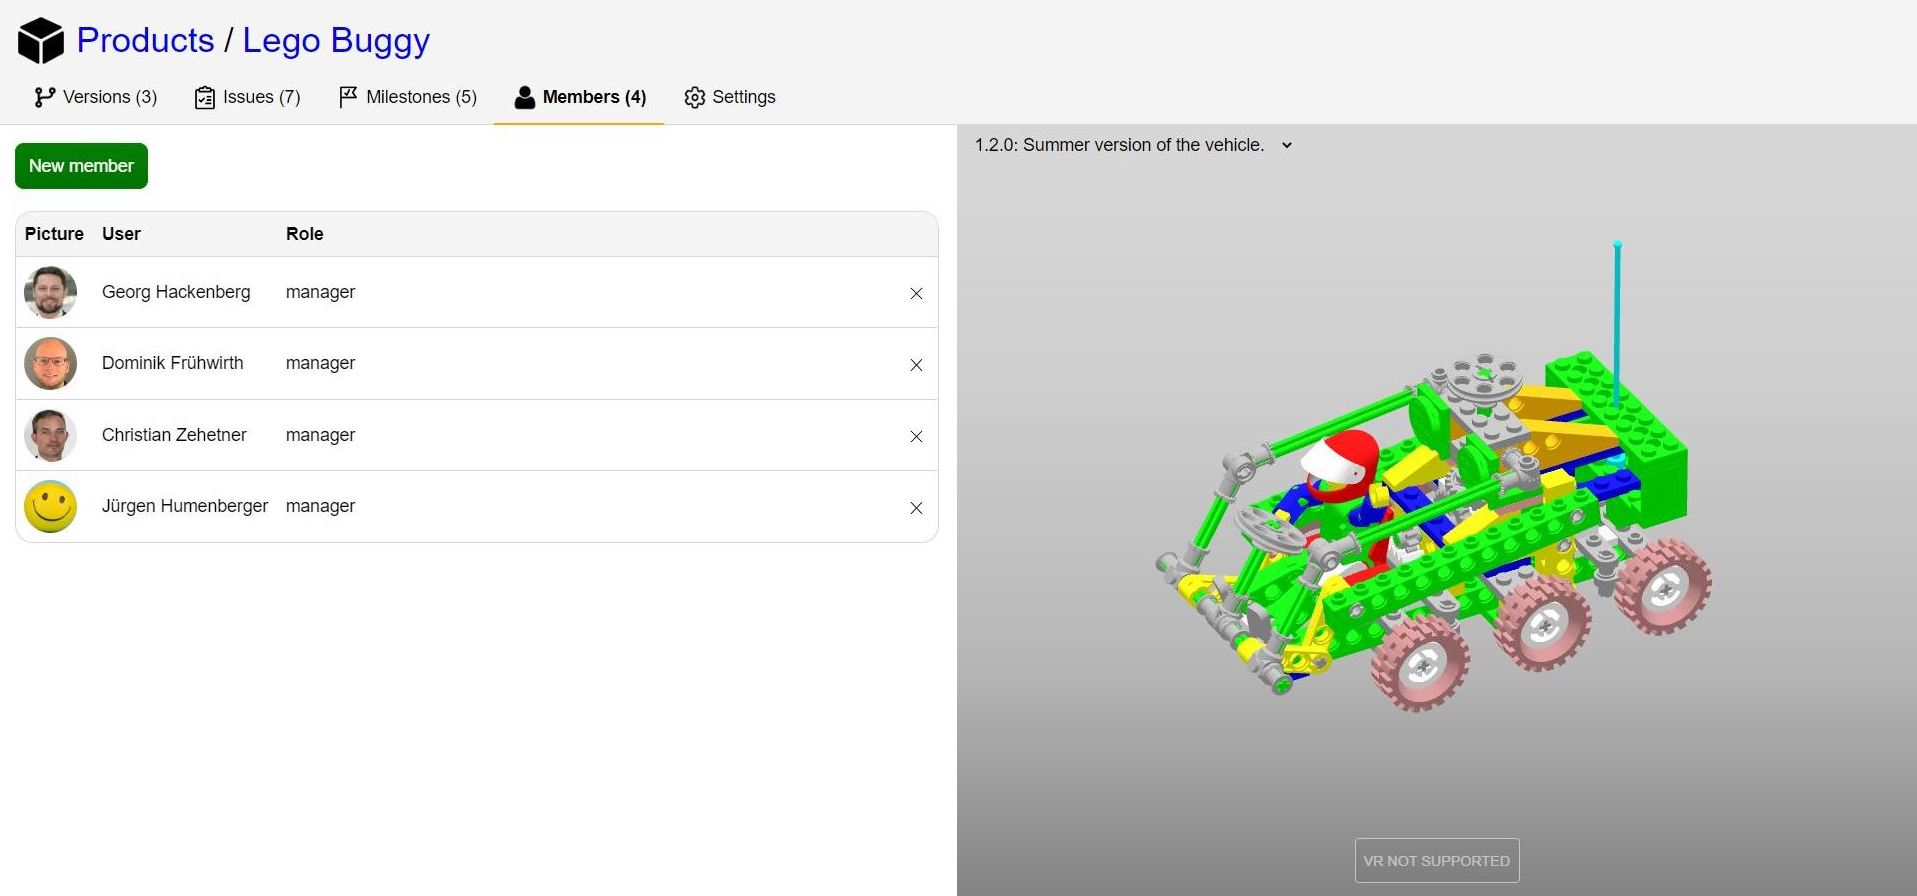
\includegraphics[width=\columnwidth]{memberview.JPG}
    \caption{Member view}
    \label{fig: memberview}
\end{figure}